% ============================================================================================
% SUPPLEMENTAL MATERIAL for the PRL draft (prl/main.tex). Skeleton started 2026-10-14.
% Role: everything the PRL states in one sentence gets its evidence here. Order follows the main text.
% Each section: lead sentence (paper register) + "%% CONTENT" list with numbers and sources (theory report section, scripts, runs)
% + figure slots reusing the report's vector figures (S-numbered). "TODO" = decision or missing piece.
% Sources: reports/theory_report (2026-10-14), RESEARCH.md, reports/master (methods detail).
% ============================================================================================
\documentclass[aps,prl,onecolumn,superscriptaddress,amsmath,amssymb,nofootinbib]{revtex4-2}
\usepackage{graphicx}
\usepackage{xcolor}
\usepackage[hidelinks]{hyperref}
\graphicspath{{../../theory_report/figs/}}
\DeclareGraphicsExtensions{.pdf,.png}
\newcommand{\half}{\tfrac12}
\newcommand{\la}{\ell_a}
\newcommand{\kT}{k_BT}
\newcommand{\todo}[1]{\textcolor{red}{[TODO: #1]}}
% S-numbering for figures, tables, equations and sections
\renewcommand{\thefigure}{S\arabic{figure}}
\renewcommand{\thetable}{S\arabic{table}}
\renewcommand{\theequation}{S\arabic{equation}}
\renewcommand{\thesection}{S\arabic{section}}

\begin{document}
\title{Supplemental Material for ``Flow alignment sets the topological charge of active nematic cavities''}
\author{Benjamin Loewe}
\affiliation{Facultad de F\'isica, Pontificia Universidad Cat\'olica de Chile, Santiago 7820436, Chile}
\author{Tyler N. Shendruk}
\affiliation{School of Physics and Astronomy, The University of Edinburgh, Peter Guthrie Tait Road, Edinburgh EH9 3FD, United Kingdom}
\maketitle
\tableofcontents

% ============================================================================================
\section{Simulation method and parameters}\label{si:methods}
Simulations use the active-nematic multi-particle collision dynamics (AN-MPCD) of Ref.~\cite{Kozhukhov2022} in two dimensions.
%% CONTENT (source: master 01_model.tex):
%%  - Units: cells a, mass m, kBT = 1; time unit tau_0 (written t.u.); density 20 per cell; collision operator 21 (dipolar activity + nematic Andersen rotation),
%%    nematic mean-field strength U_MF = 10, flow-alignment (Bretherton) parameter lambda (2 unless stated; < 1 tumbling); grid shift.
%%  - Activity zeta = 0.07 (working value) and why: below 0.05 onset effects, above 0.09 compressibility (Mach ~ 1); active length l_a = 22.2 +- 0.3 cells
%%    measured as sqrt(area/<N>) in periodic boxes (100^2, 200^2) [Kozhukhov2024]. Table S1: l_a vs zeta.
%%  - Walls: no-slip bounce-back; anchoring theta = k phi as ghost-particle orientation (strong anchoring), uniform in arclength for ellipses/ovals; cavity shapes
%%    (circle radius R; ellipses aspect eps; Cassini ovals; R_eq = sqrt(area/pi)); periodic channel (flat limit) with walls >= 1 cell inside the domain.
%%  - Frank constants K1 ~ 42, K3 ~ 23 kBT (how measured); rotational viscosity gamma_1 ~ 60 kBT t.u./cell^2 (director-mode decay); free-defect mobility 0.0054.
%%  - Run list: Table S2 (geometry, k, lambda, seeds, steps, outputs) for every data set in the main text.
\begin{table}[h]\caption{\todo{Table S1: active length vs activity}}\end{table}
\begin{table}[h]\caption{\todo{Table S2: data sets (cavity, $k$, $\lambda$, size, seeds, duration, output intervals)}}\end{table}

\section{Defect detection and observables}\label{si:observables}
%% CONTENT: defect tracker (topological charge on the cell grid; positions on the grid, half/sixth cells from cluster averages); head/tail convention
%% (defects.dat angle = direction of div Q = tail of a +1/2; bulk +1/2 move against it, 66-72 % of steps); wall layer = +1/2 within 4 cells (justification Sec. S10);
%% wall count, bulk charge Q_b (net charge beyond 4 cells), tilt tau_j (tail vs outward normal), tilt coherence C = |<e^{i tau_j}>|, circulation <v_phi>,
%% two-vortex criterion (halves counter-rotate), vacancies, escape (band -> 6 cells deep) and depleting escape, control defects.

% ============================================================================================
\section{Overcharged circles: size and winding}\label{si:circles}
%% CONTENT: wall count and bulk charge vs R/l_a for k = 2..10 (server production, 10 seeds) -> TODO new Fig. S1 from runs/cavity (server);
%% onset R/l_a ~ 0.8 for the full layer, tilt/circulation onset 0.4-0.6; fraction of time in the overcharged state; half-integer k (odd layers 3, 5, 9; k = 1.5 no layer);
%% negative winding (seeded starts: active 13.5 / 13.0 wall -1/2 of 14 predicted, passive relaxes to 12) -> open point.
\begin{figure}[h]
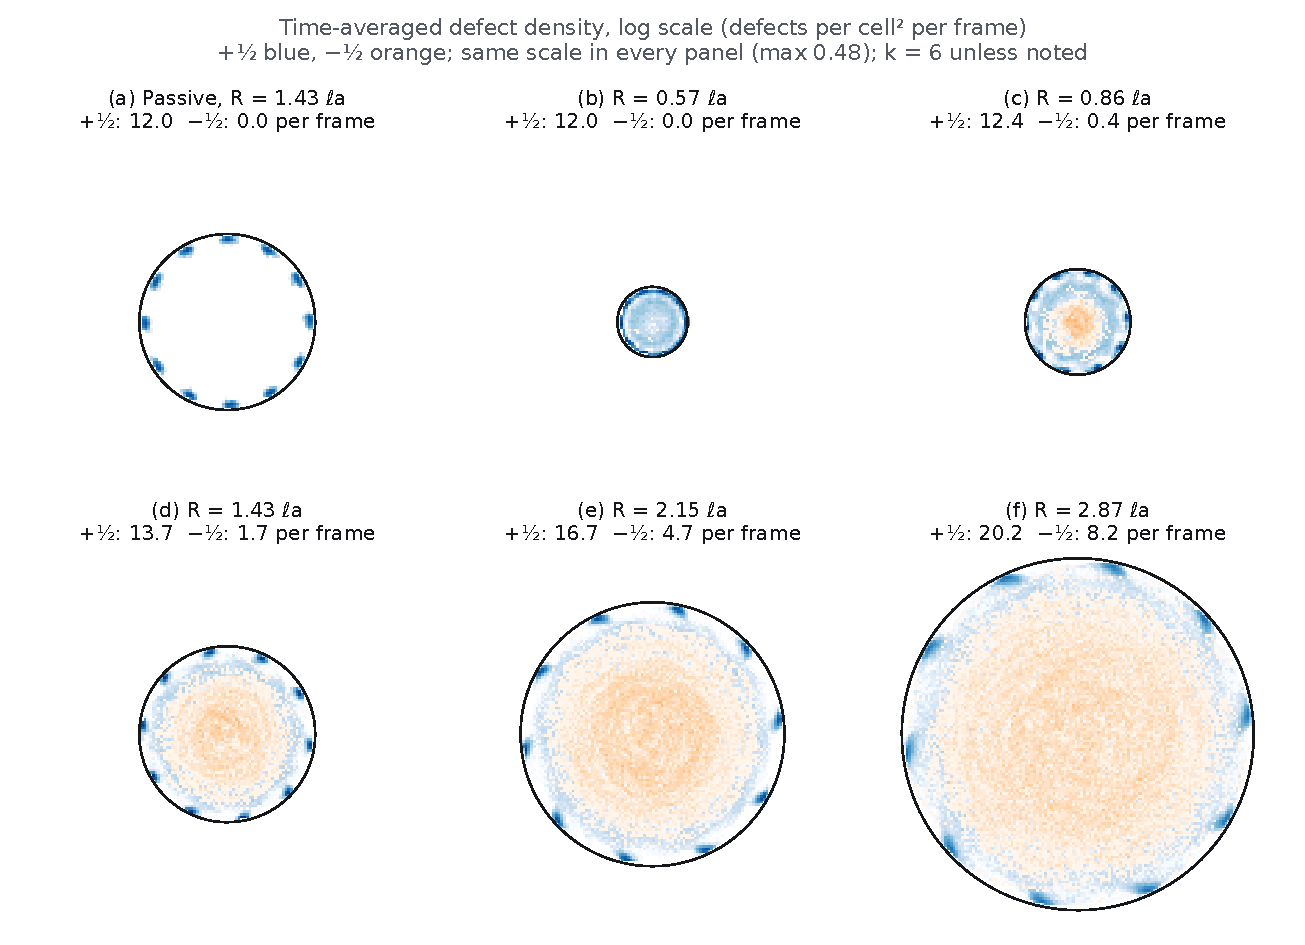
\includegraphics[width=0.8\textwidth]{maps_circles}
\caption{\todo{Fig.~S1}: density maps; to be joined by wall count and bulk charge vs $R/\la$ and $k$ (production runs).}\label{fig:s_maps}
\end{figure}

% ============================================================================================
\section{Anchoring geometry, the lock and pinning}\label{si:lock}
%% CONTENT: derivation of the (2k-2)-fold symmetry and of tau_j = (2k-2) phi_j + const; local version for arbitrary walls (psi_rel(s) = 2 pi k s/P - phi_n(s));
%% measured lock (mean resultant 0.99; 0.91-0.99 in every shape); commensurability (2k ring tilts wind twice; measured -60 deg steps);
%% pinning by K1 != K3: barrier 80-110 kBT (active 2k-2 ring) vs < 1 kBT (passive 2k ring); initial-condition tests (6 directors, registry 0.03 +- 0.07);
%% sine-modulated winding moves the sites (0.21-0.27 cells); fluctuations: harmonic (Hessian) theory reproduces the along-wall rms within 2-4 %.
\begin{figure}[h]
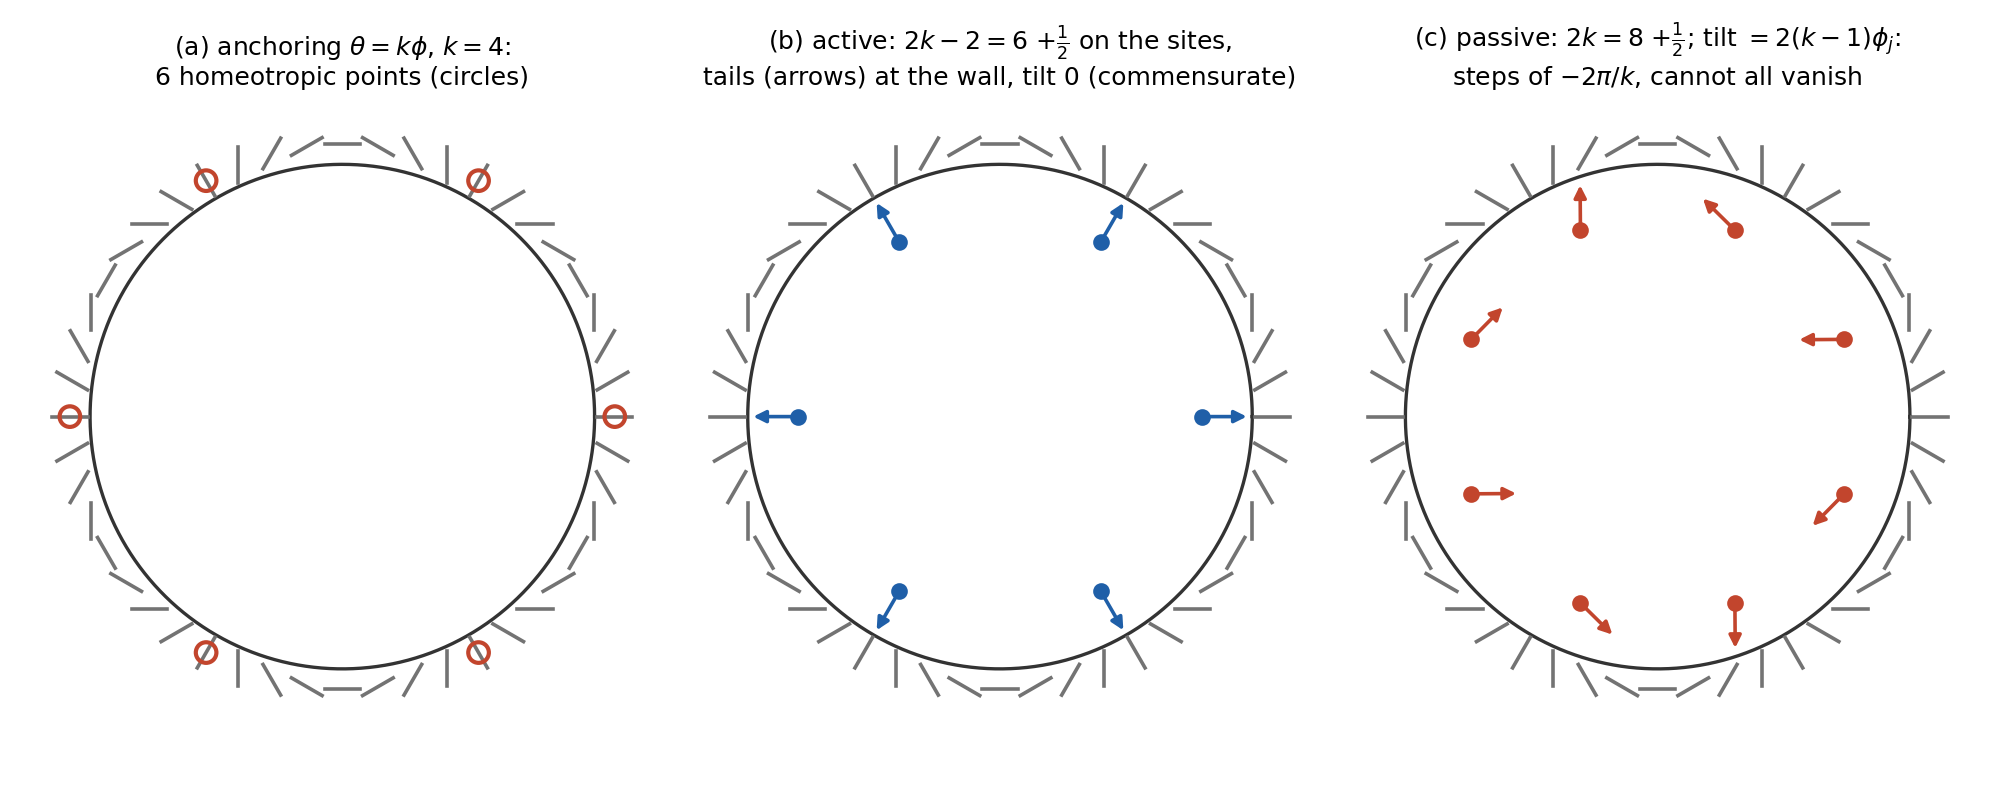
\includegraphics[width=0.8\textwidth]{fig_lock}
\caption{\todo{Fig.~S2} (if not in the main text): anchoring sites and the tilt--position lock.}\label{fig:s_lock}
\end{figure}

% ============================================================================================
\section{Elastic energetics of ejection}\label{si:energy}
%% CONTENT: point-defect Frank energy in the anchored disk (method of images; anisotropic K1/K3 to second order; relaxed cores); energies:
%% eject without flow +155..200 kBT; common tilt on the 2k ring +200..500; ejected structure tilts at -38..+3; net favourable by 170-300 under a common tilt.
\begin{figure}[h]
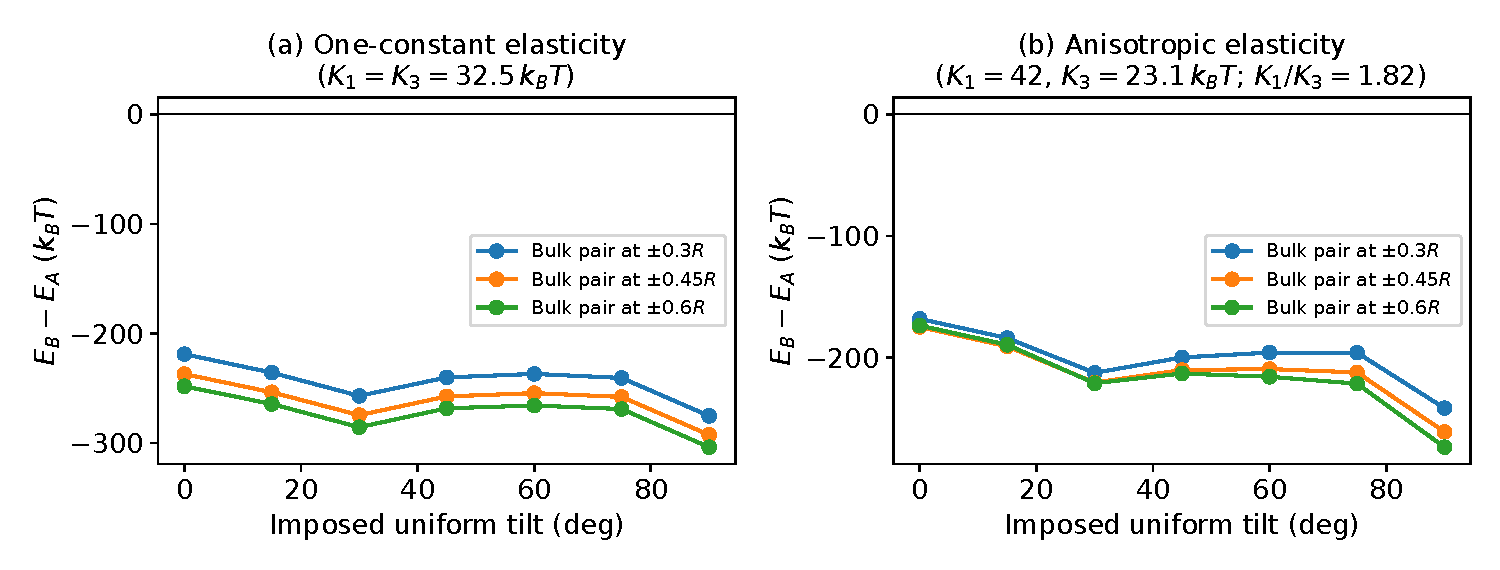
\includegraphics[width=0.8\textwidth]{tilted_structures}
\caption{\todo{Fig.~S3}: energy of the ejected structure minus the $2k$ ring under a common tilt, one-constant and anisotropic.}\label{fig:s_energy}
\end{figure}

% ============================================================================================
\section{Passive cavities under an imposed vortex}\label{si:swirl}
%% CONTENT: body-force implementation (azimuthal acceleration A, solver branch); runs (A, lambda, seeds); threshold A ~ 0.003-0.01; needs a common tilt (C > 0.9) and
%% flow alignment (lambda 0.5 never, 1.2 partly); tilt 57-68 deg (lambda 2), 75-83 (4); active layer under an imposed reversal is stick-slip (lock-sized jumps).
\begin{figure}[h]
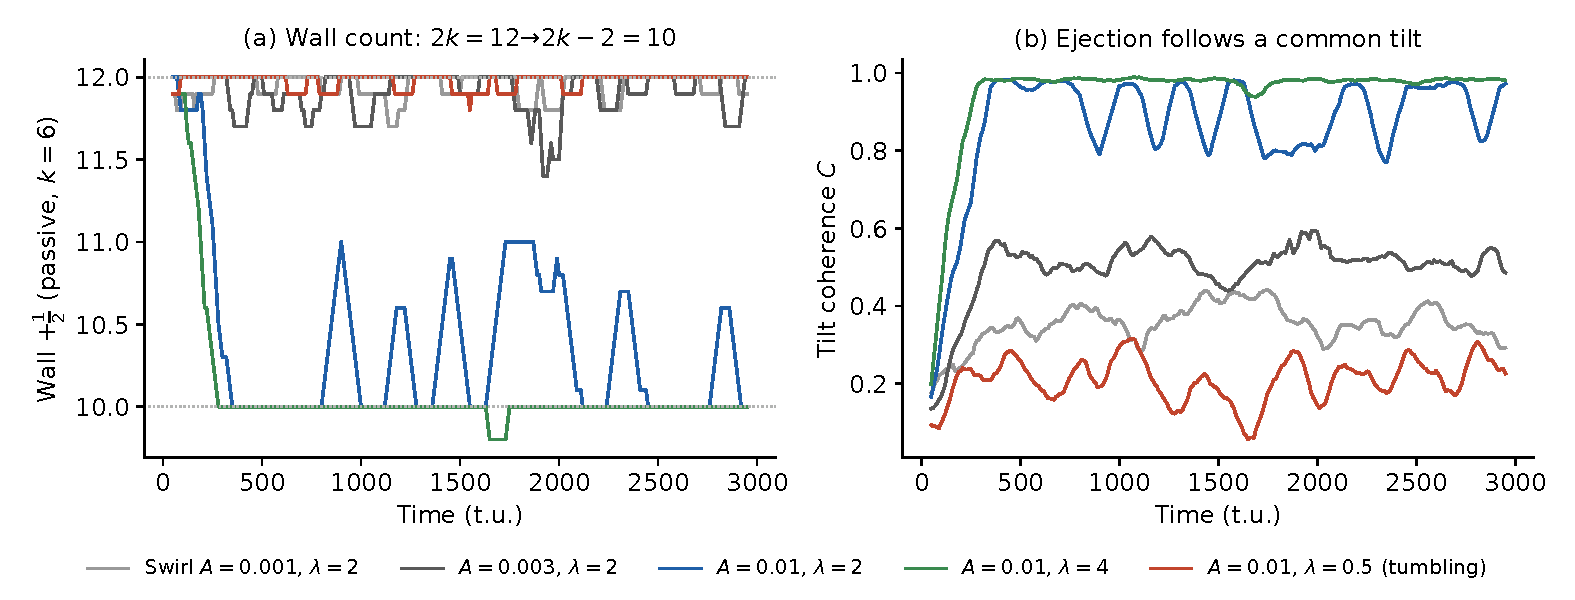
\includegraphics[width=0.8\textwidth]{fig_ejection}
\caption{\todo{Fig.~S4}: passive cavity under an imposed vortex (full time series, all amplitudes).}\label{fig:s_swirl}
\end{figure}

% ============================================================================================
\section{Continuum models}\label{si:continuum}
\subsection{Passive Q-tensor with the measured flow}
%% CONTENT: Beris-Edwards equations, parameters (L = a = Gamma = 1, S_eq 0.876, lambda_c = lambda S_eq), imposed flow v_theta = U f(r) from the MPCD swirl profile;
%% results: threshold, tilt 65-67 deg (lambda 2), 78-79 (4); flow-profile variants (shear only in / removed from the wall band). Fig. shear_tilt.
\subsection{Active Q-tensor with Stokes backflow}
%% CONTENT: model (extensile stress, one constant), disk: zeta 0.1 vortex without ejection, 0.3 and 1.0 eject, tilt 61.7-62.1 deg; ellipses: transition at 1.4-1.6 (Fig. fig_cont_ellipse).
\subsection{Flat-wall theory}
%% CONTENT: Ericksen-Leslie with winding anchoring (kappa = pi/a_s); zero mode; leading order arccos(1/lambda); boundary-layer correction (ansatz) and its test (35 runs).
\begin{figure}[h]
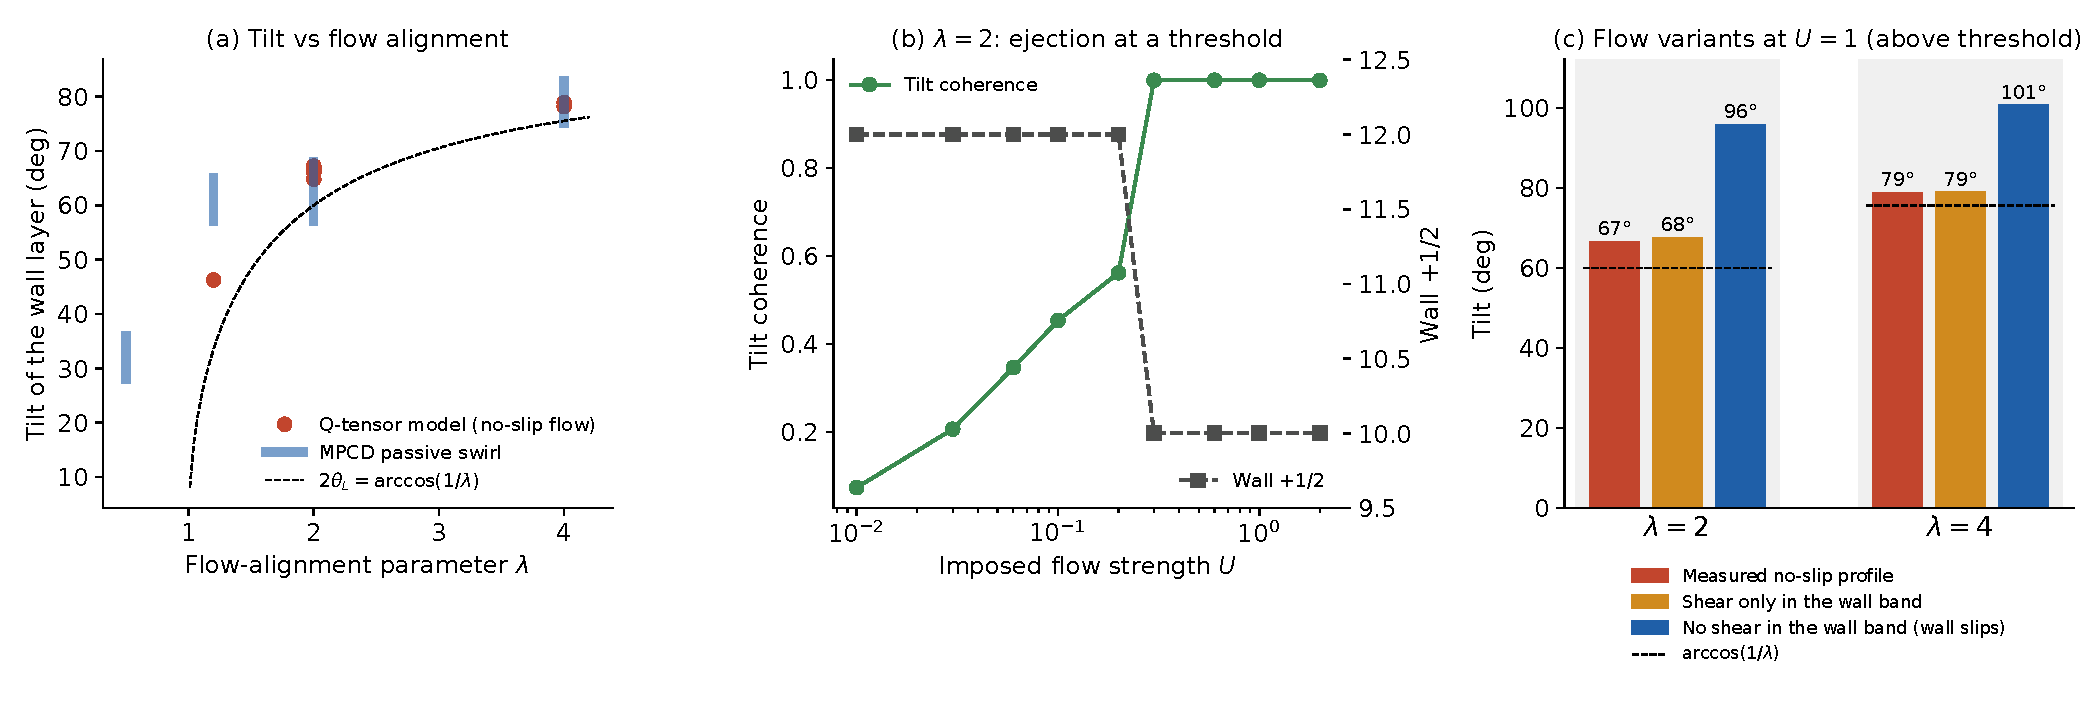
\includegraphics[width=0.8\textwidth]{shear_tilt}
\caption{\todo{Fig.~S5}: passive Q-tensor model with the measured flow.}\label{fig:s_qtensor}
\end{figure}
\begin{figure}[h]
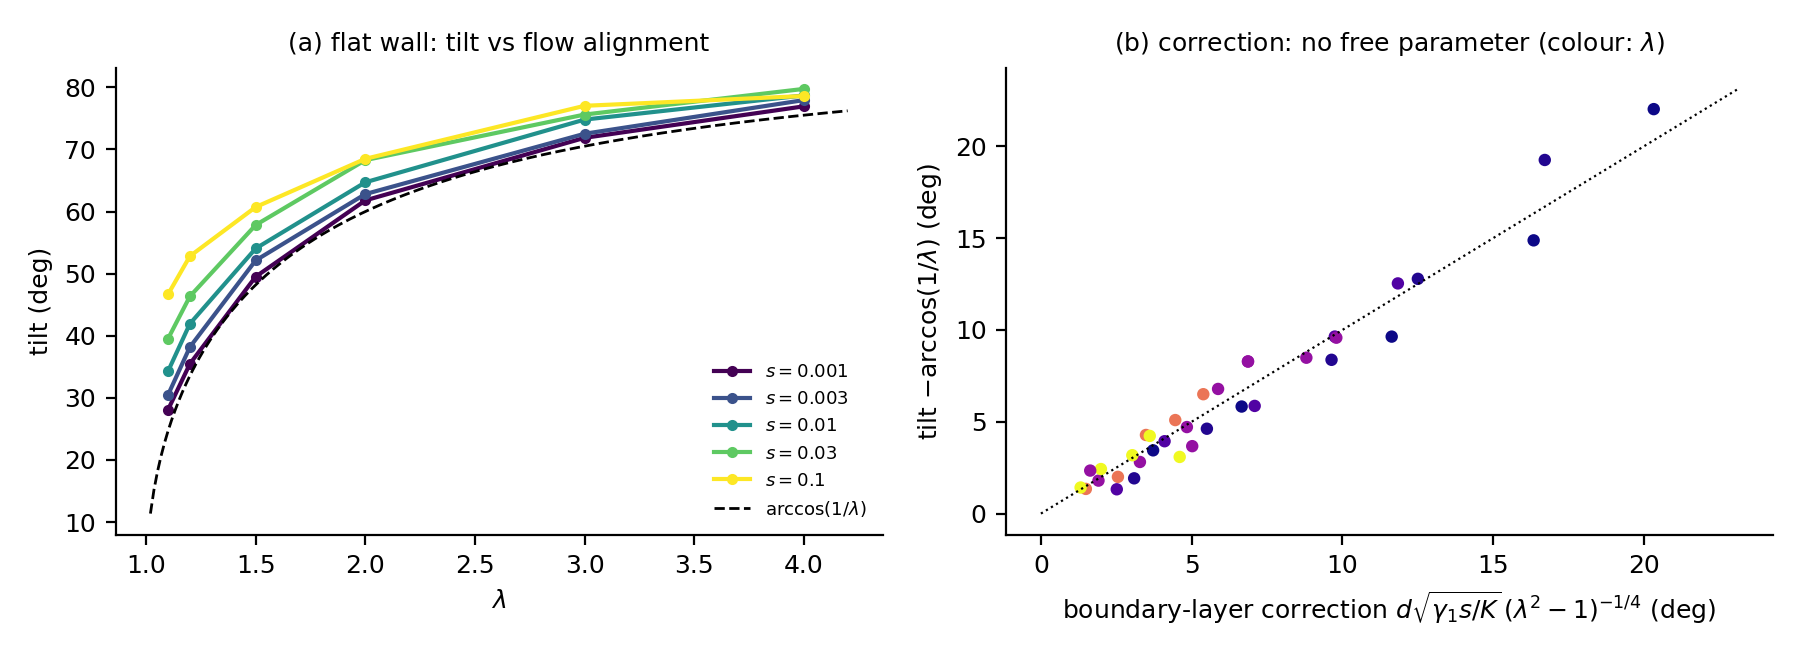
\includegraphics[width=0.8\textwidth]{fig_flatwall}
\caption{\todo{Fig.~S6}: flat-wall theory test.}\label{fig:s_flatwall}
\end{figure}

% ============================================================================================
\section{The tilt in MPCD: mechanism and residuals}\label{si:tilt}
%% CONTENT: director rotation at the defects' depth = Leslie angle (26-33 deg), tilt = 2x; lambda scan details (seeds, k = 4, 6, 8; table of tilts);
%% breakdown below lambda ~ 2: wall count, coherence, escapes; size dependence (runs/lamsize, TODO when batch 2 is in);
%% residual vs lambda (+3 -> -2.5 deg): boundary layer absent (would be +16 deg), order-dependent alignment (sheared-channel Leslie angle vs U_MF; lambda_eff), splay != bend (+2-3 deg).
\begin{figure}[h]
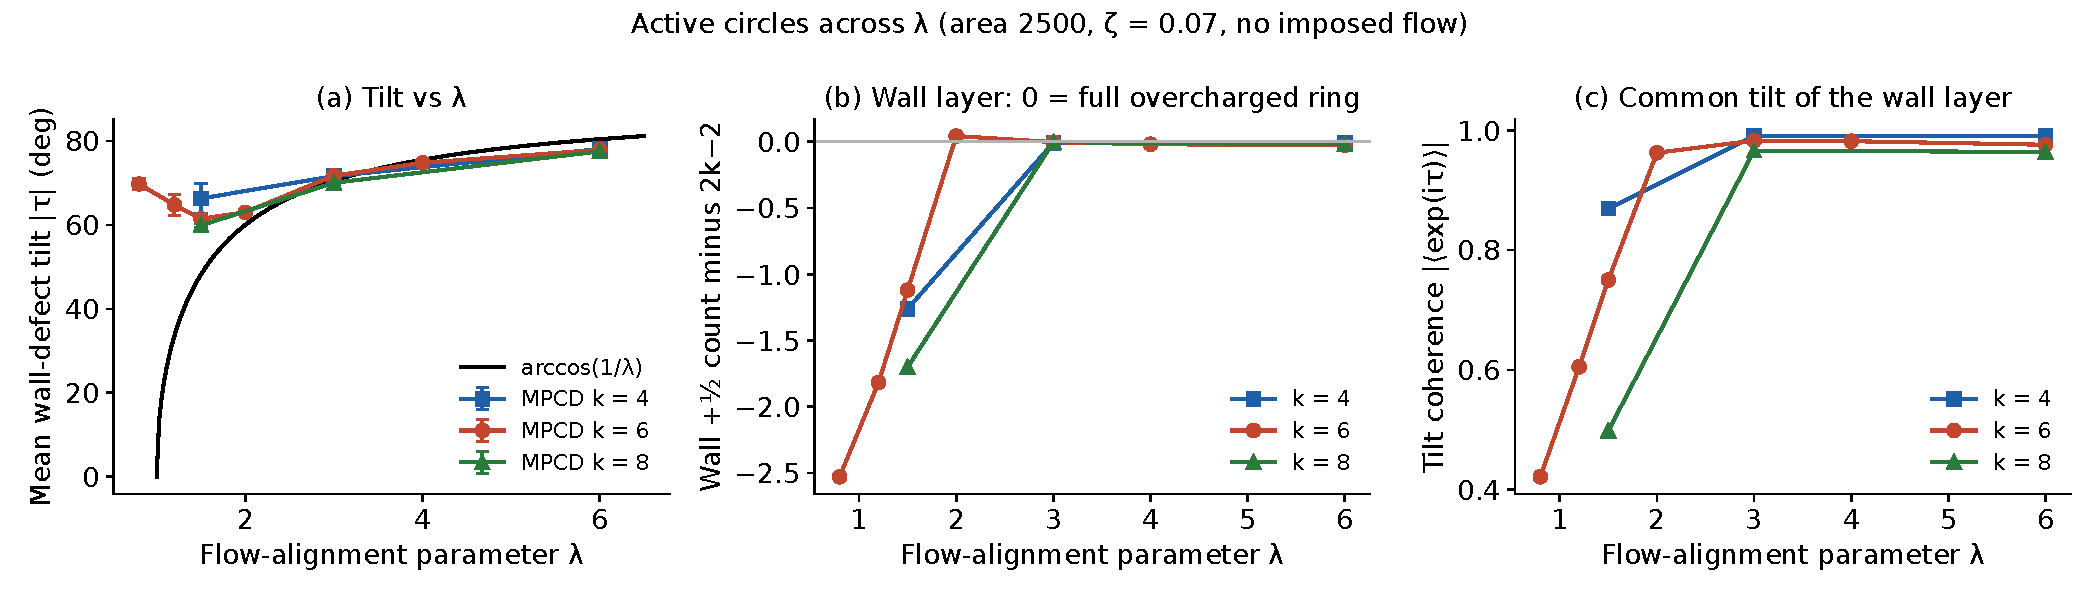
\includegraphics[width=0.8\textwidth]{fig_tiltlaw}
\caption{\todo{Fig.~S7}: full tilt-law data (all $k$, wall count and coherence).}\label{fig:s_tiltlaw}
\end{figure}

% ============================================================================================
\section{Where the flow comes from}\label{si:hydro}
%% CONTENT: director-field Stokes model (f = -div Q, wall band vs bulk, one c per run; R^2 0.48-0.72; bulk drives, wall band opposes, common scale);
%% the layer as an effective planar winding-1 boundary (site pattern fades as e^{-2 pi delta/l}; spiral offset c = 90 + tau/2); linear stability -> onset R/l_a 0.4-0.6;
%% why point-defect hydrodynamics fails (6-21 %), Langevin particle model.
\begin{figure}[h]
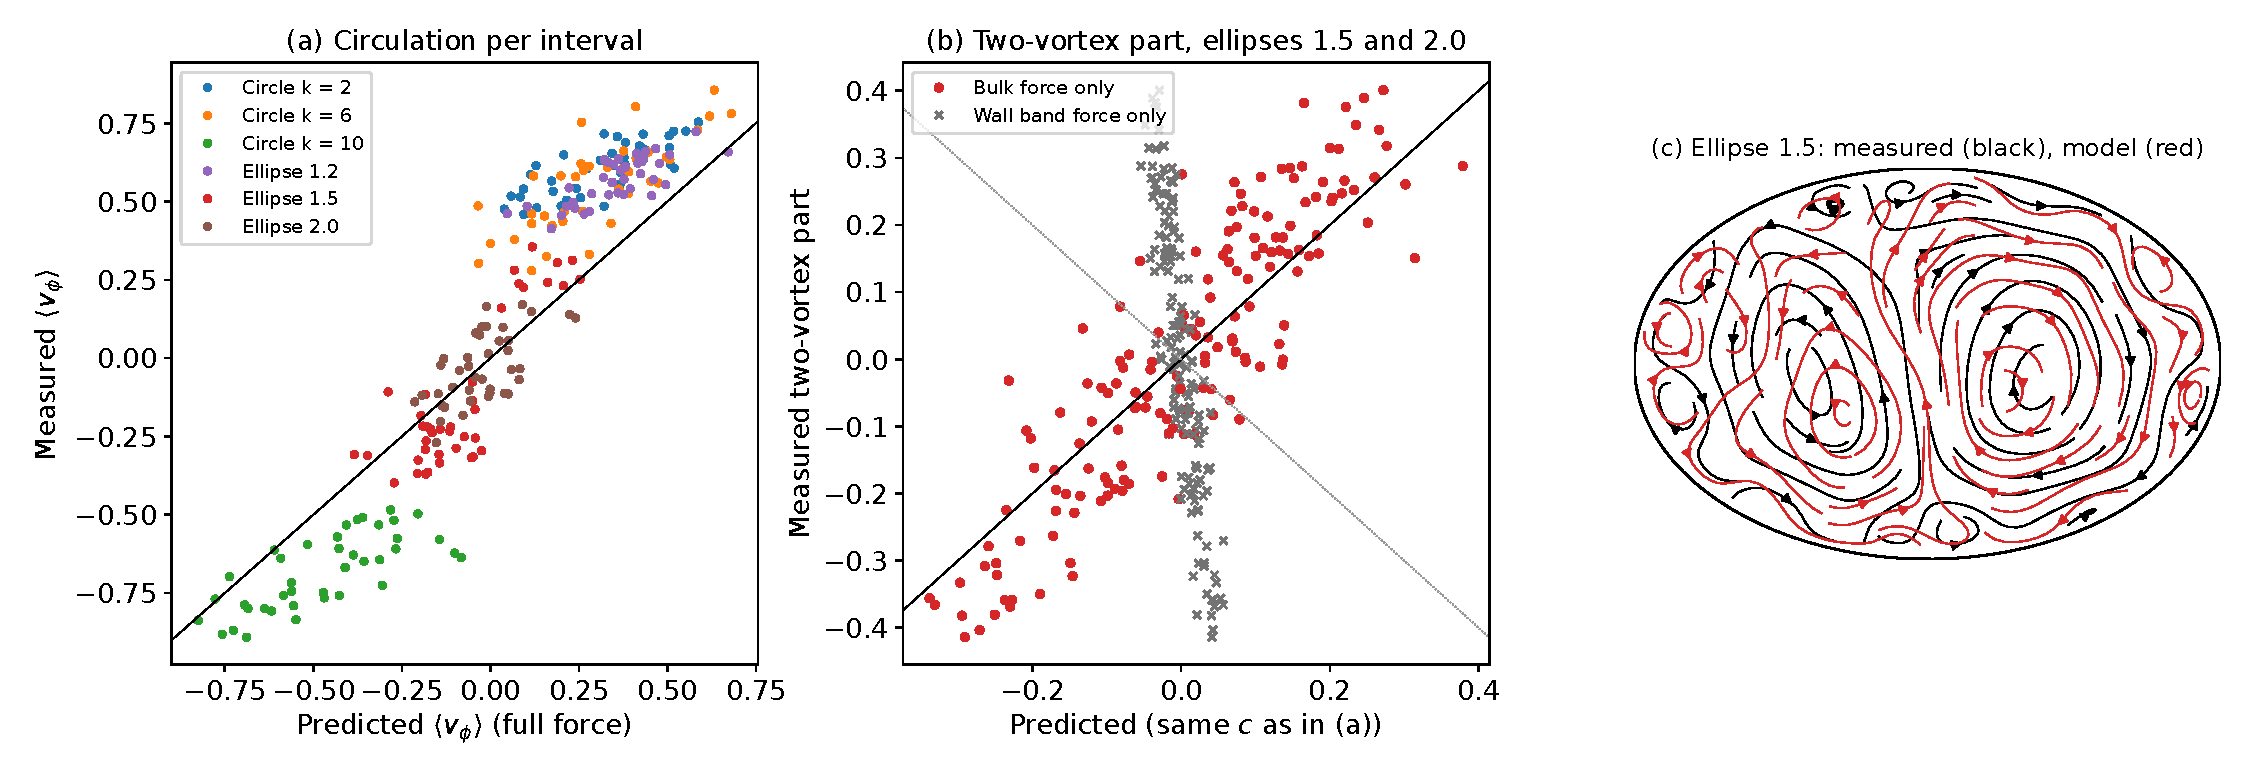
\includegraphics[width=0.8\textwidth]{dirstokes}
\caption{\todo{Fig.~S8}: director-field Stokes model.}\label{fig:s_stokes}
\end{figure}
\begin{figure}[h]
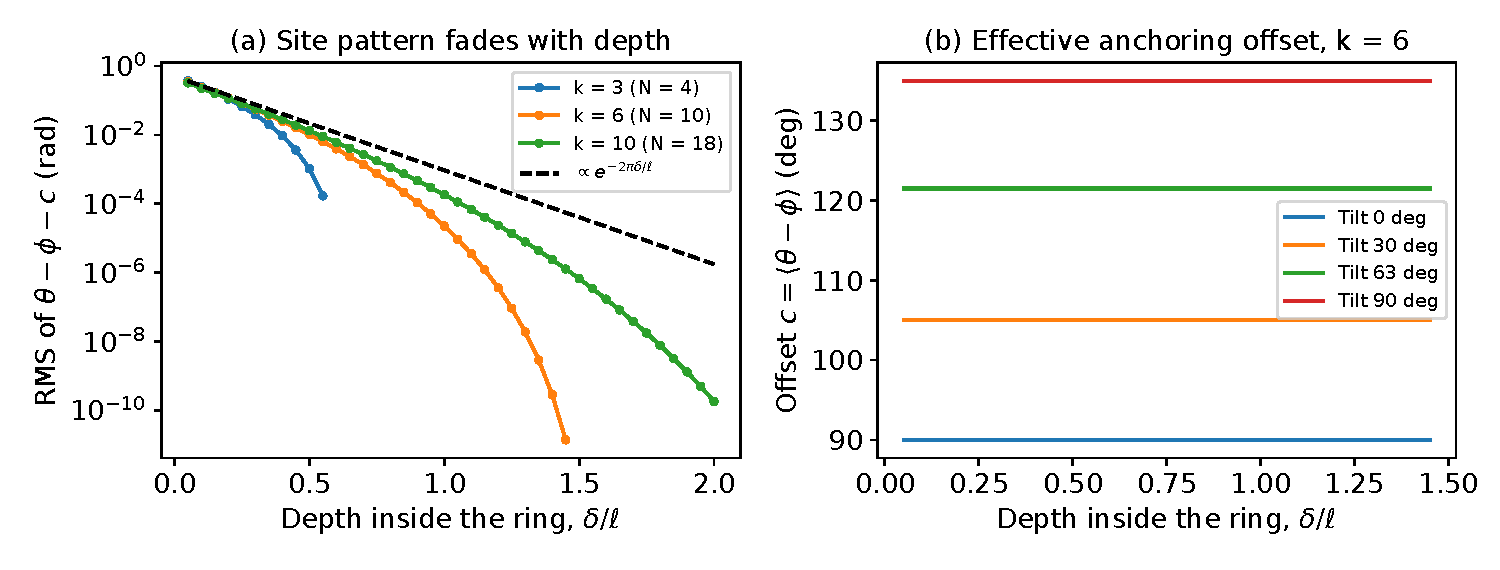
\includegraphics[width=0.8\textwidth]{effective_bc}
\caption{\todo{Fig.~S9}: the layer as an effective boundary.}\label{fig:s_effbc}
\end{figure}

% ============================================================================================
\section{Elongated cavities}\label{si:shapes}
%% CONTENT: shape sweep (675 runs; families, sizes, k, densities); phase diagram (transition at aspect 1.25-1.37, scale-free; ellipses = ovals);
%% layer loss is escape-driven, refill not starved, no cascade (Fig. fig_shapes_mech); effective restoring force collapses, elastic part unchanged (Fig. fig_restoring);
%% activity layout test (activity only in the wall band keeps the coherent state; only in the bulk breaks it, even in circles); imposed swirl in active ellipses.
\begin{figure}[h]
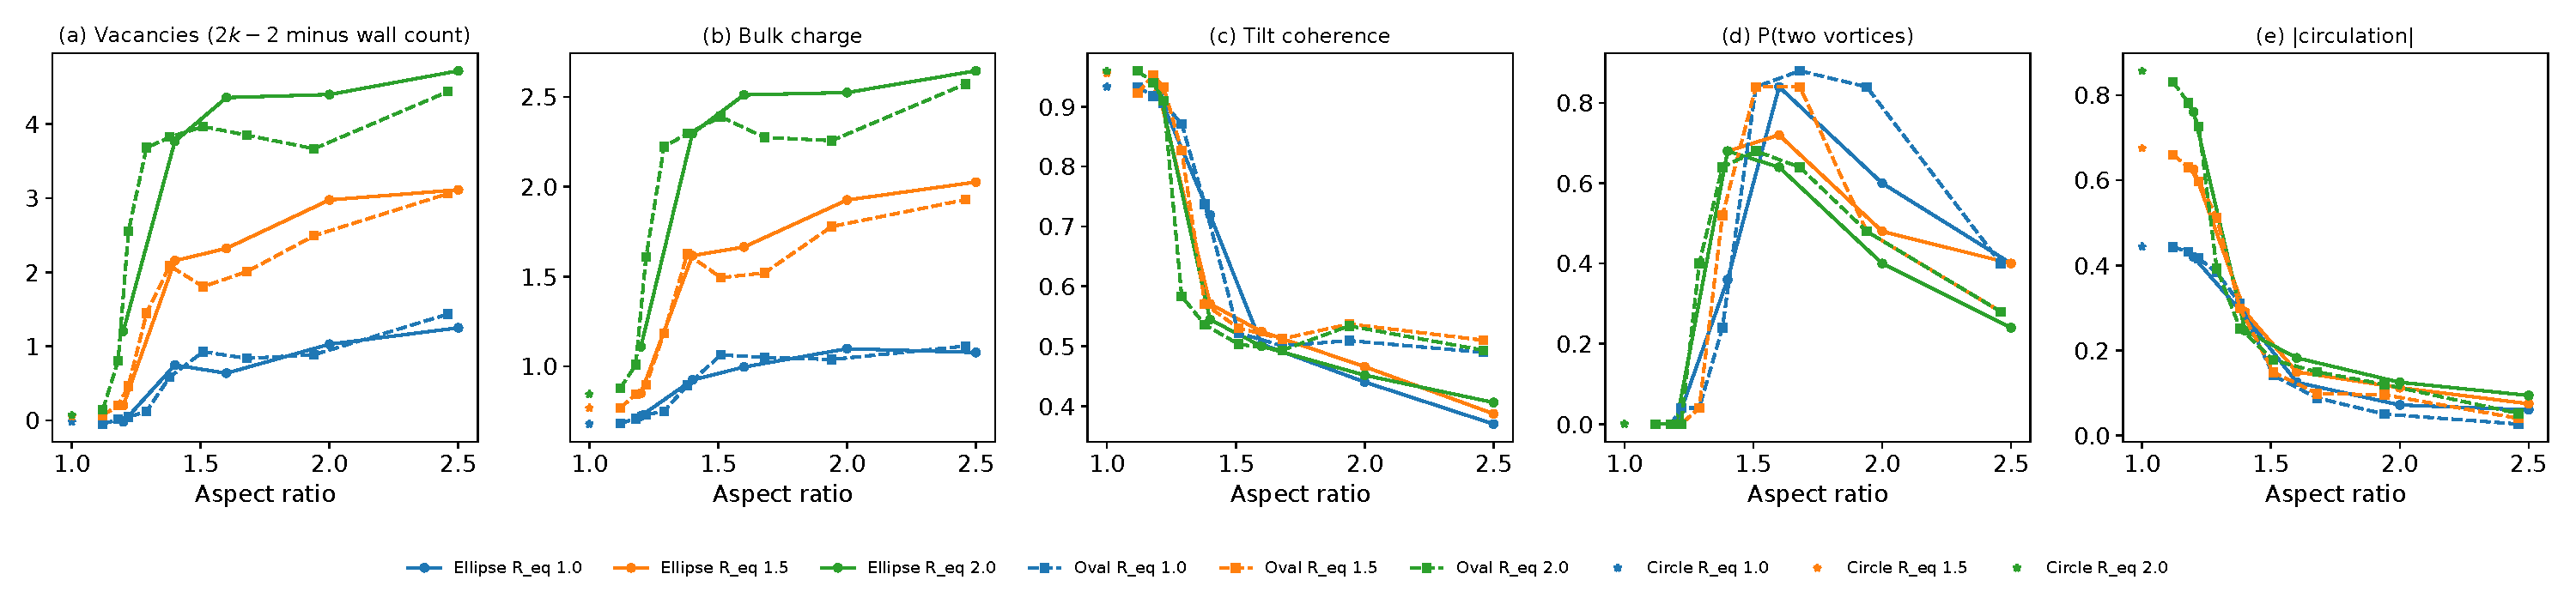
\includegraphics[width=\textwidth]{phase_shapes}
\caption{\todo{Fig.~S10}: shape sweep phase diagram.}\label{fig:s_phase}
\end{figure}
\begin{figure}[h]
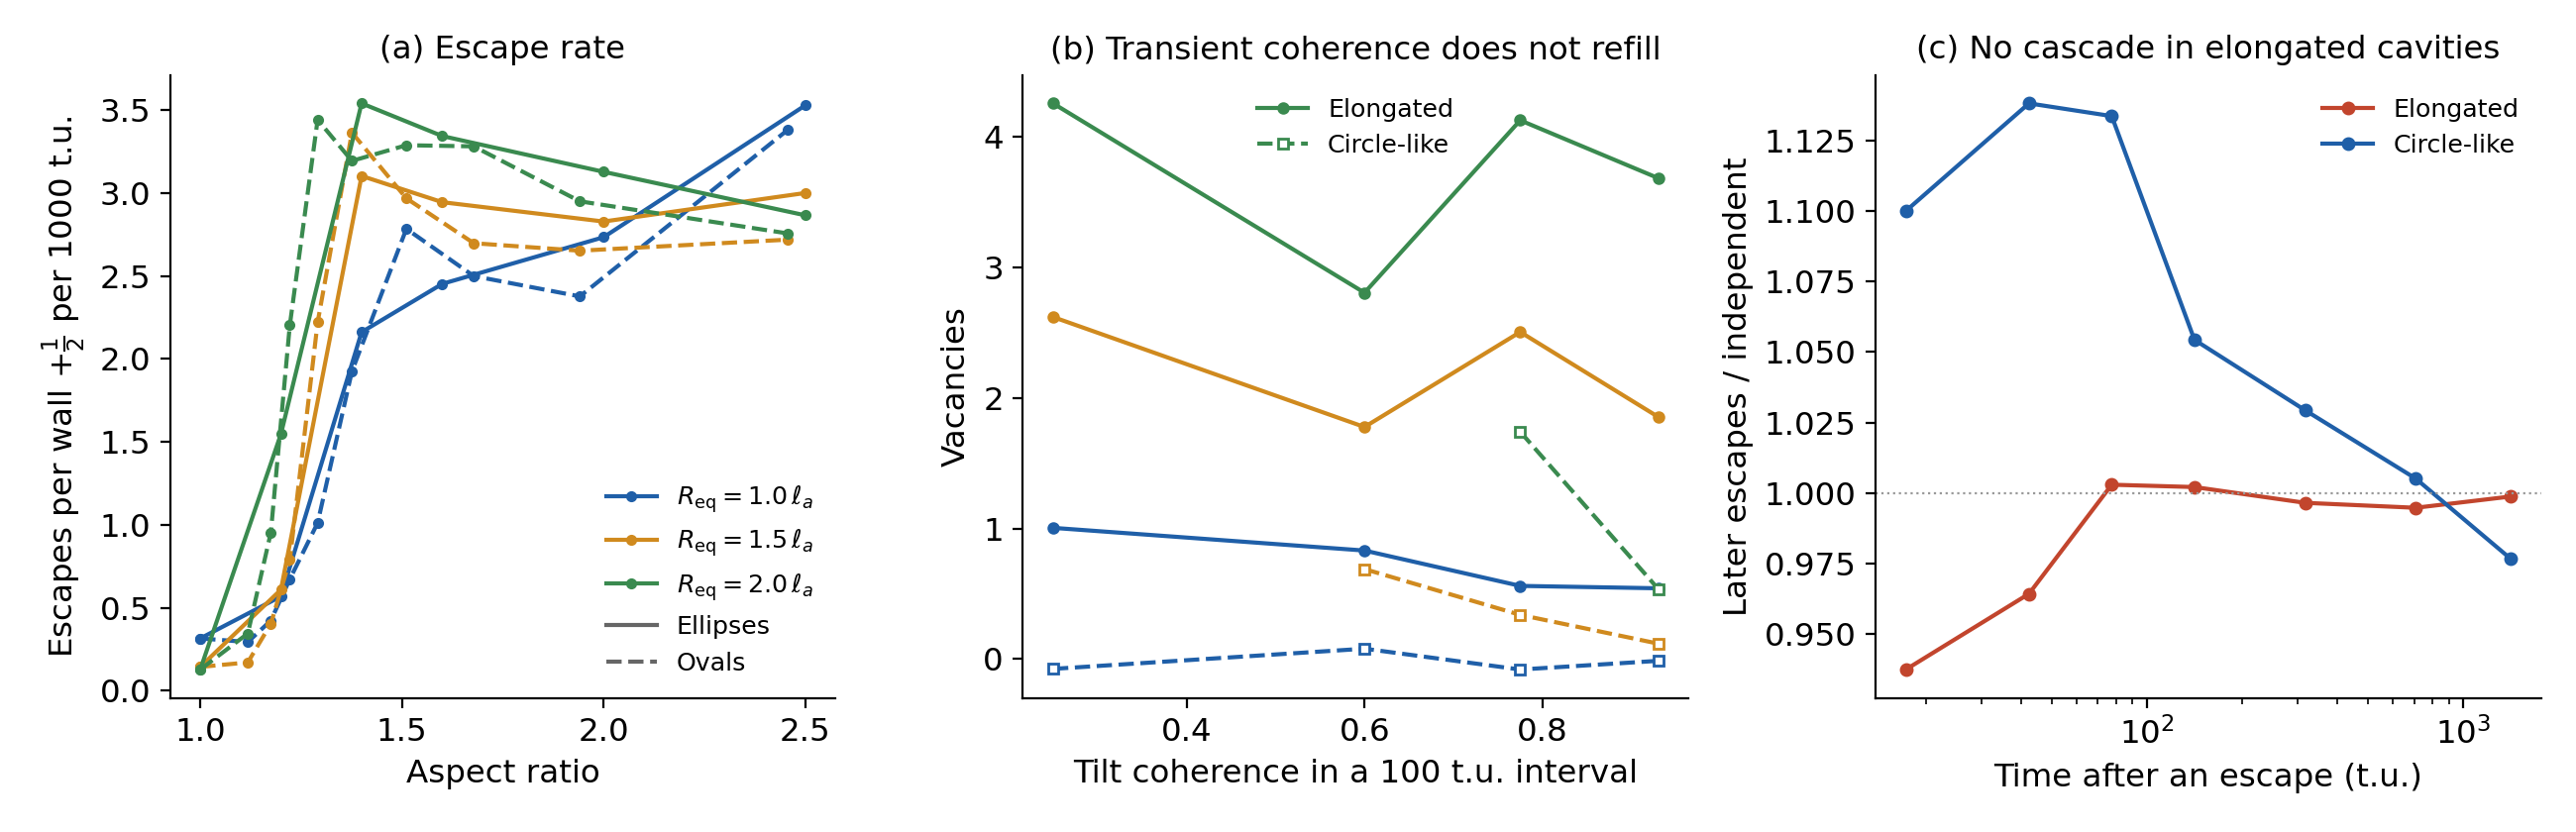
\includegraphics[width=0.8\textwidth]{fig_shapes_mech}
\caption{\todo{Fig.~S11}: escape-driven, non-cascading layer loss.}\label{fig:s_mech}
\end{figure}

% ============================================================================================
\section{How a wall defect leaves}\label{si:escape}
%% CONTENT: event selection (depleting escapes, 11-12 % of all; alignment on departure; 36 fine-flow runs, 411 events; controls);
%% elastic barrier intact (F0 -11..-14 kBT/cell, Fig. fig_etsg_shapes); untilting and own jet (Fig. fig_selfflow); the wall blocks the normal jet component,
%% g(d) = 0.30/0.33/0.58/0.86/1 and the closed law 0.40 cos(tau) g(d) (Fig. fig_jetmap); wall-side lobe erased and recovering (Fig. fig_vortdef);
%% landing on viscometric (Q = 0) lines [Head2024] (Fig. fig_qcrit); force balance (alpha 0.87, beta 0.98, mu_n 0.0016); tips vs flanks (Fig. fig_etsg_reg);
%% passive wall band: jet-free route (Fig. fig_compare_bulk); untilting is driven (Langevin null model); precursors at -40 t.u.; Movie S1 (escape with lobe overlay).
\begin{figure}[h]
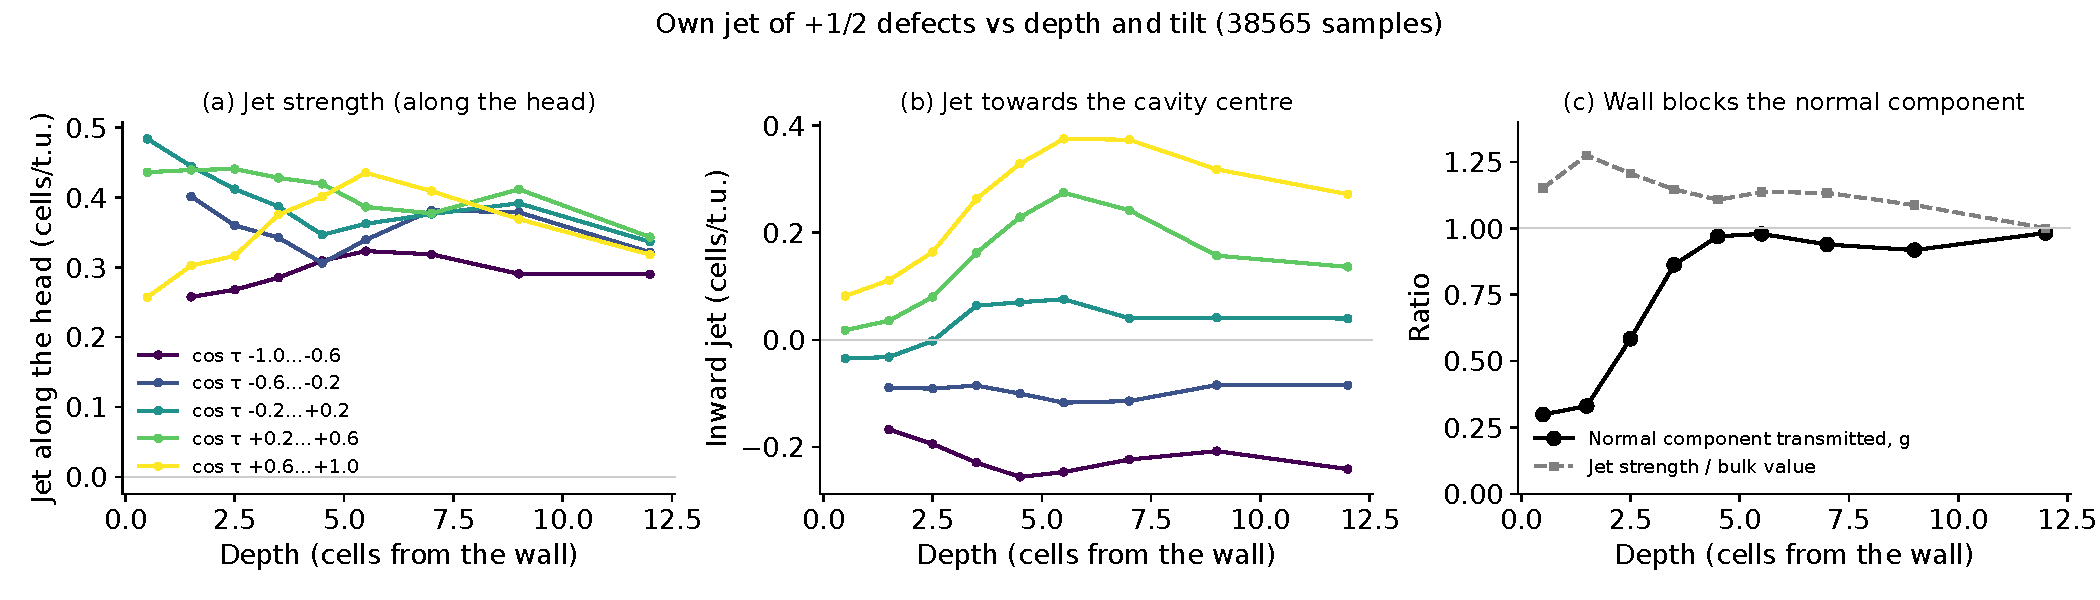
\includegraphics[width=0.8\textwidth]{fig_jetmap_ff12}
\caption{\todo{Fig.~S12}: the own jet and its wall blocking (with Figs.~S13--S15: run-up, lobes, viscometric lines).}\label{fig:s_jet}
\end{figure}

% ============================================================================================
\section{Mirror control: negative winding}\label{si:mirror}
Reversing the winding ($k\to-k$) puts $-\half$ defects in the wall layer; they are not self-propelled, so they test whether the leak of elongated cavities is
driven by the wall defects' own jets.
%% CONTENT (TODO: server mirror shape sweep, 675 runs = same cavities as the +k sweep, starts after the circle seeds; analysis = shape_sweep_analysis + perlength
%% with sign-aware wall counts):
%%  - circles: commensurate -1/2 ring has 2|k-1| = 2|k|+2 defects; energetics favour gaining two -1/2 under a common tilt (196-392 kBT minus pair creation);
%%    passive gains only at lambda 4; seeded starts (runs/neglayer): active 13.5 (circle) / 13.0 (aspect 2) of 14, unique from 12 and 14 starts, bulk +0.5..+0.7;
%%    passive 14 + bulk +1 relaxes to 12 -> MPCD vs continuum difference, open (candidate: pair creation/annihilation noise).
%%  - shapes: wall count, vacancies/excess, bulk charge, tilt coherence, two-vortex fraction vs aspect for -k vs +k (Fig. S_mirror); escape rates of wall -1/2;
%%    effective restoring force (preliminary 1 size, 2 seeds: pull-back -1.8..-2.2 at 2.5-3 cells, passive -2.6..-3.3; layers hold at eps <= 1.2).
%%  - wall law for -k? (released charge per unit length, sign).
\begin{figure}[h]
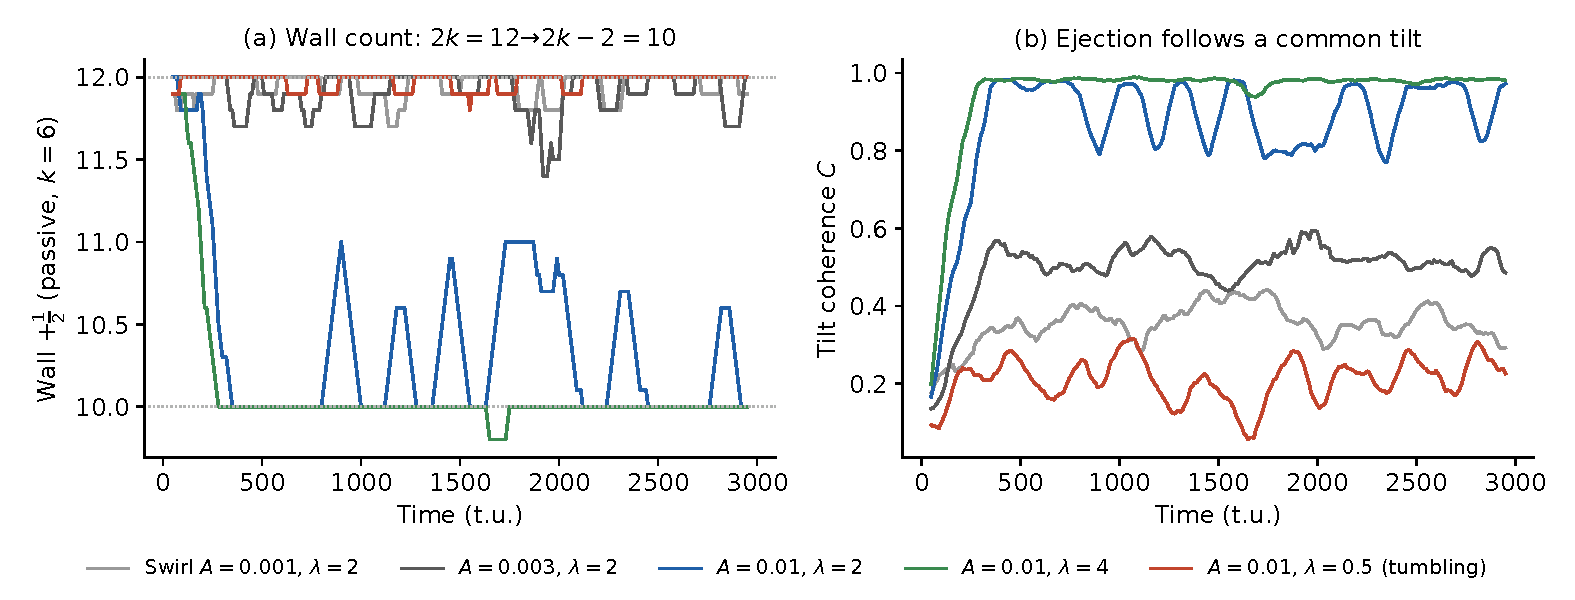
\includegraphics[width=0.6\textwidth]{fig_ejection}
\caption{\todo{Fig.~S\_mirror (placeholder image): $+k$ vs $-k$ in the same cavities: wall layer, bulk charge and coherence against aspect ratio; restoring force of wall $\pm\half$.}}\label{fig:s_mirror}
\end{figure}

% ============================================================================================
\section{Steady state and the wall law}\label{si:steady}
%% CONTENT: lambda test (exits and refills slowed together); depleted layer far above the elastic optimum (-80..-100 kBT per refill; Cassini model -81..-89);
%% unique steady state from seeded starts (4/7/10 -> 7.2; seeding method); self-limitation by crowding (exit rate 0.068 -> 0.028 per 20 t.u.);
%% wall law: bulk charge per unit length vs aspect and q (Fig. fig_perlength), area^0.47 at fixed q; periodic channel as the flat limit (Fig. fig_channel; widths 18-60 hold the
%% same share, narrower channels break down).
\begin{figure}[h]
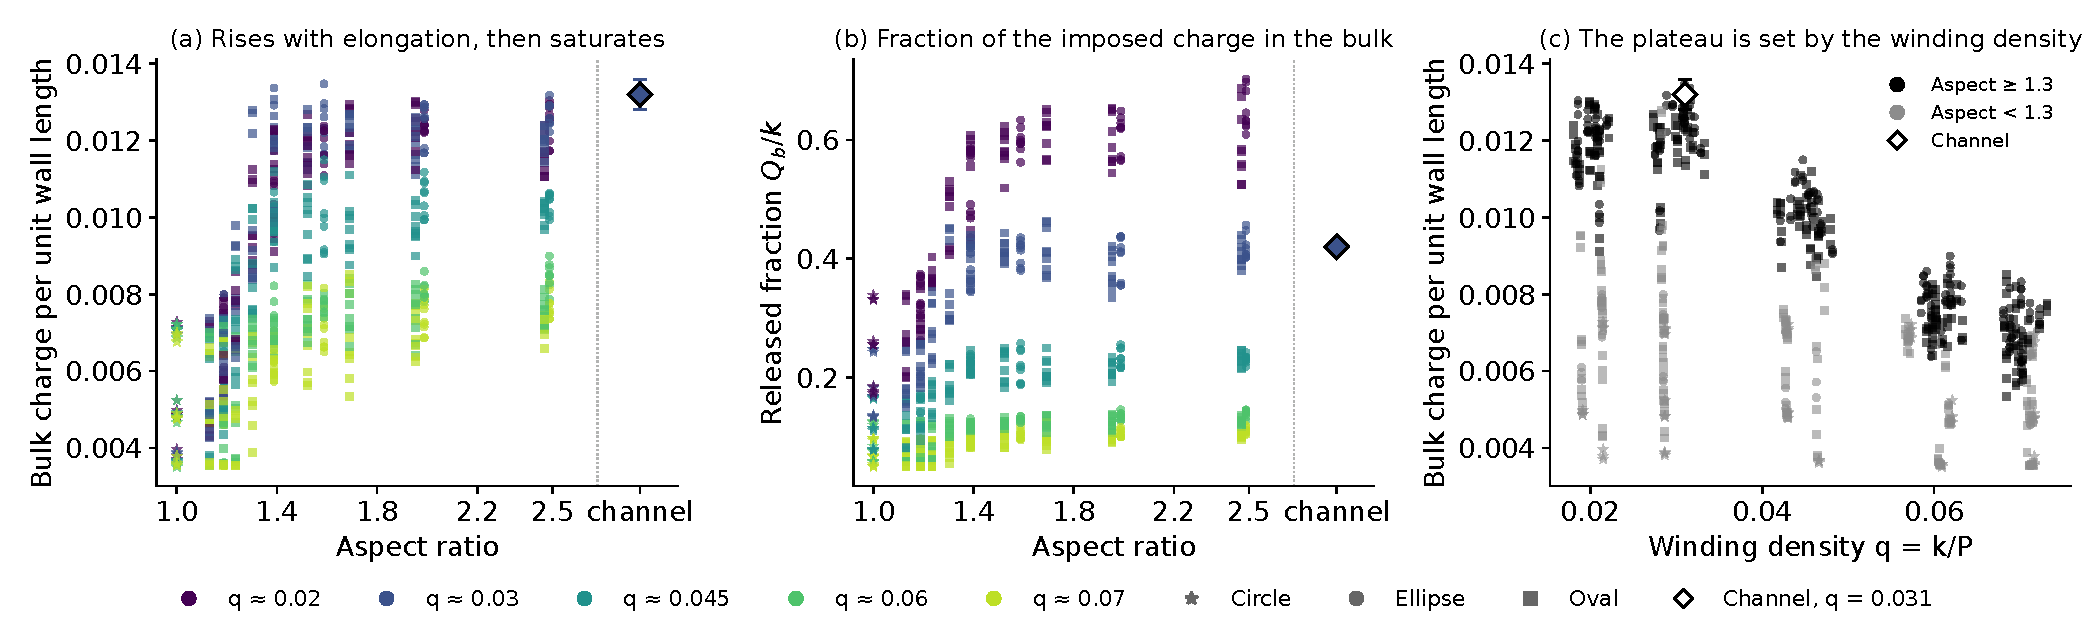
\includegraphics[width=\textwidth]{fig_perlength}
\caption{\todo{Fig.~S16} (or main Fig.~4c): the wall law with all runs.}\label{fig:s_walllaw}
\end{figure}
\begin{figure}[h]
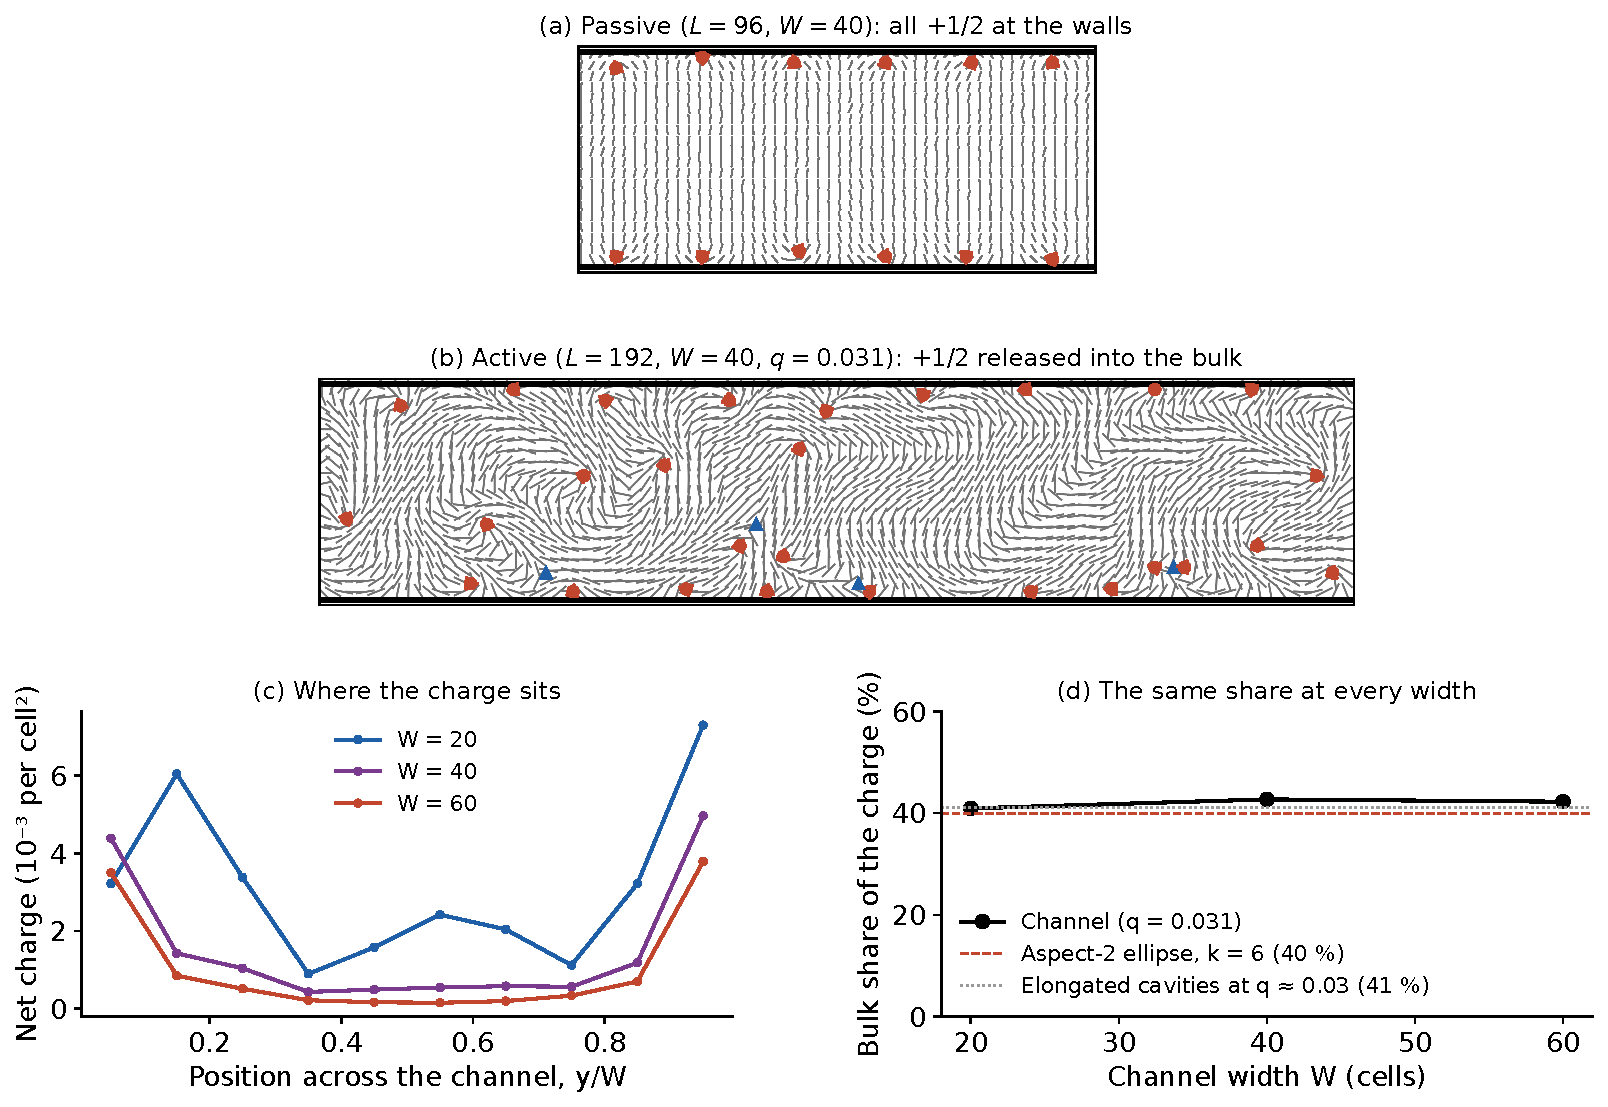
\includegraphics[width=0.8\textwidth]{fig_channel}
\caption{\todo{Fig.~S17}: the periodic winding channel, flat limit of the wall law.}\label{fig:s_channel}
\end{figure}

% ============================================================================================
\section{Layer versus bulk defects}\label{si:layer}
%% CONTENT: justification of the 4-cell criterion: depth distribution, mobility crossover at 3-5 cells, weak site locking in channels; robustness to 3 or 5 cells.
\begin{figure}[h]
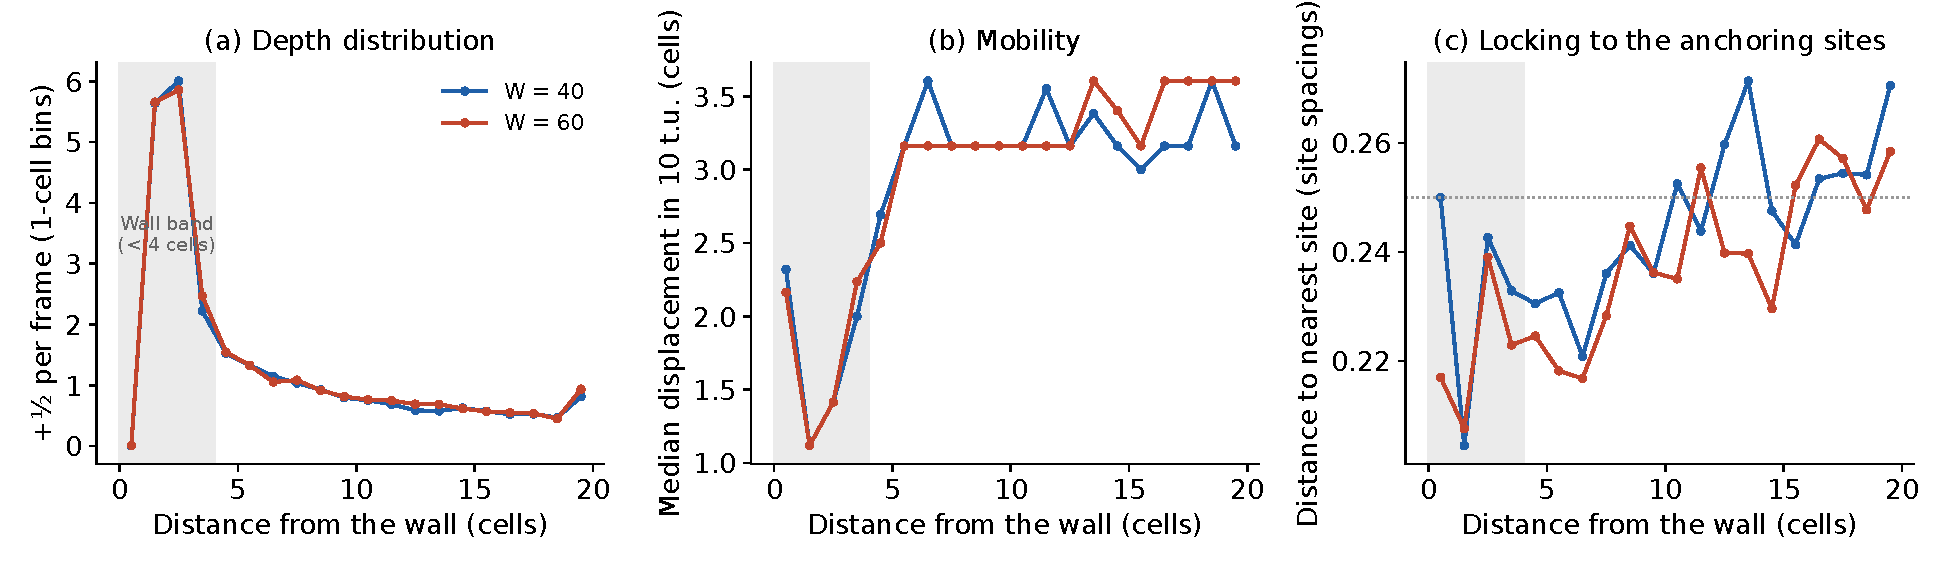
\includegraphics[width=0.8\textwidth]{fig_layer_profile}
\caption{\todo{Fig.~S18}: $+\half$ defects by distance from the wall.}\label{fig:s_layer}
\end{figure}

% ============================================================================================
\section{Movies}\label{si:movies}
%% CONTENT: Movie S1 active circle (k = 6): overcharged state, tilted layer, single vortex. Movie S2 passive cavity under an imposed vortex: ejection.
%% Movie S3 escape event in an aspect-2 ellipse with the vortex-lobe overlay (movie/escape_eps2.0_s2_ev4.mp4). Movie S4 periodic channel (flat limit). TODO: make S1, S2, S4.

\bibliography{../refs}
\end{document}
